\documentclass[10pt,portuguese]{article}
\usepackage[portuguese]{babel}

\usepackage{fourier}
\usepackage[bottom]{footmisc}

\usepackage[]{graphicx}
\usepackage[]{color}
\usepackage{xcolor}
\usepackage{alltt}
\usepackage{listings}
\usepackage[T1]{fontenc}
\usepackage[utf8]{inputenc}
\setlength{\parskip}{\smallskipamount}
\setlength{\parindent}{5ex}
\usepackage{indentfirst}
\usepackage{listings}
\usepackage{setspace}
\usepackage{hyperref}
\hypersetup{
    colorlinks=true,
    linkcolor=auburn,
    filecolor=magenta,      
    urlcolor=blue, 
    urlsize=2em
}

\usepackage{tabto}

% Set page margins
\usepackage[top=100pt,bottom=100pt,left=68pt,right=66pt]{geometry}

% Package used for placeholder text
\usepackage{lipsum}

% Prevents LaTeX from filling out a page to the bottom
\raggedbottom

\definecolor{javared}{rgb}{0.6,0,0} % for strings
\definecolor{javagreen}{rgb}{0.25,0.5,0.35} % comments
\definecolor{javapurple}{rgb}{0.5,0,0.35} % keywords
\definecolor{javadocblue}{rgb}{0.25,0.35,0.75} % javadoc

\lstset{language=Java,
basicstyle=\footnotesize\ttfamily,
keywordstyle=\color{javapurple}\bfseries,
stringstyle=\color{javared},
commentstyle=\color{javagreen},
morecomment=[s][\color{javadocblue}]{/**}{*/},
numbers=left,
numberstyle=\tiny\color{black},
stepnumber=2,
numbersep=10pt,
tabsize=4,
showspaces=false,
showstringspaces=false}


\usepackage{fancyhdr}
\fancyhf{} 
\fancyfoot[C]{\thepage}
\renewcommand{\headrulewidth}{0pt} 
\pagestyle{fancy}

\usepackage{titlesec}
\titleformat{\chapter}
   {\normalfont\LARGE\bfseries}{\thechapter.}{1em}{}
\titlespacing{\chapter}{0pt}{50pt}{2\baselineskip}

\usepackage{float}
\floatstyle{plaintop}
\restylefloat{table}

\usepackage[tableposition=top]{caption}


\definecolor{light-gray}{gray}{0.95}

\renewcommand{\contentsname}{Índice}

\begin{document}


\begin{titlepage}
	\clearpage\thispagestyle{empty}
	\centering
	\vspace{2cm}

	
	{\Large  Compiladores \par}
	\vspace{0.5cm}
	{\small Miguel Oliveira e Silva\par
	Artur Pereira\par}
	\vspace{3cm}
	{\huge \textbf{Linguagem para análise dimensional: \\ Chubix}}
	\vspace{1cm}
	\vspace{4cm}
	{\normalsize  \par Bruno Bastos, 93302 \par 
	Hugo Almeida, 93195 \par
	Mário Silva, 93430
	\par Leandro Silva, 93446 
	   \par Rui Fernandes, 92952}
	 
	\vspace{2cm}

    
\includegraphics[scale=0.20]{images/logo_ua.png}
    
    \vspace{2cm}
    
	{\normalsize DETI \\ 
		Universidade de Aveiro \par}
		
	{\normalsize \today \par}
	\vspace{2cm}
		
	
	\pagebreak

\end{titlepage}
\tableofcontents{}
\clearpage

%%%%%%%%%%%%%%%%%%%%%%%%%%%%%%%%%%%%%%%%%%%%%%%%%%%%%%%%%%%%%%%%%%%%%%%
\section{Introdução}

\par Este documento visa descrever e guiar o leitor por todo o processo de desenvolvimento do projeto final da unidade curricular de Compiladores. O trabalho foi desenvolvido pelos estudantes identificados na capa sendo que recorreram maioritariamente à assistência do docente Prof. Dr. Miguel Oliveira e Silva.
\par Este projeto tem como principal objetivo o desenvolvimento de um compilador assente em duas linguagens, uma para o compilador em si, e outra complementar que auxilia o funcionamento da primeira. Ao longo do desenvolvimento tentou-se ao máximo seguir todas as fases de construção de linguagens de programação.
\par Foram utilizadas as tarefas e métodos aprendidos nas aulas da unidade curricular, o ANTLR4 e programação em Java.
\par O grupo decidiu escolher como tema para o projeto, um dos temas sugeridos no guião do trabalho, sendo este o desenvolvimento de uma linguagem de programação para análise Dimensional. Este tema tem por base estender o sistema de tipos de uma linguagem de programação possibilitando a definição de dimensões distintas e interoperáveis, a expressões numéricas. Sendo uma linguagem destas de grande utilidade para problemas de Física ou Química em que existem várias dimensões nas quais é preciso operar, é importante que as operações possíveis façam sentido.
\par Tendo isto em conta, foi criada uma linguagem de programação principal com as funcionalidades básicas de uma linguagem como Java ou Python com o acrescento de incorporar análise dimensional, servindo de base à construção do compilador. Desenvolveu-se também uma linguagem complementar a esta que permite criar as dimensões e unidades físicas pretendidas pelo utilizador.

%%%%%%%%%%%%%%%%%%%%%%%%%%%%%%%%%%%%%%%%%%%%%%%%%%%%%%%%%%%%%%%%%%%%%%%
\newpage
\section{Concepção e Definição da Linguagem}

\par Desde o inicio soube-se que o maior desafio seria como criar novas dimensões e unidades, e posteriormente utilizá-las e definir variáveis usando então o sistema de dimensões. Tirando isto, na linguagem principal tencionava-se incluir todas as funcionalidades básicas necessárias como instruções iterativas e condicionais, bem como funções, declaração de variáveis e todas as operações matemáticas base.
\par A sintaxe de criação de dimensões e unidades passou por várias fases no momento de idealização, o objetivo era principalmente que fosse fácil de utilizar e de entender para o utilizador. Segue-se então a evolução da mesma:
\newline
\par \textbf{1ª Fase:}
\begin{itemize}
    \item create Metro as m;
    \item create Centímetro as m*10\string^-2;
\end{itemize}
\par Este primeiro conceito é obviamente defeituoso, visto que não está a ser criada uma dimensão, mas sim duas unidades e uma relação entre elas, acrescenta-se ainda que deste modo, o centímetro não tem símbolo da unidade, e apenas um símbolo que representa a sua relação ao metro.
\newline
\par \textbf{2ª Fase:}
\begin{itemize}
    \item new dim distance;
    \item new unit distance( m : 1 );
    \item new unit distance( cm : 1/100 );
\end{itemize}
\par Nesta segunda fase, separou-se então as criações de dimensões e unidades, criando explicitamente uma dimensão com identificação primeiro, e apenas depois criar unidades para a mesma, sendo que a unidade centímetro tem agora um símbolo, mantendo a sua relação ao metro. Aqui também encontraram-se problemas, por exemplo as unidades apenas se podiam relacionar com uma unidade base passada como \emph{"1"} e faltava também diferenciação entre dados \emph{Integer} e \emph{Double}.
\newline
\par \textbf{Sintaxe Final:}
\begin{itemize}
    \item dim Distance( m : Double );
    \item unit Distance( cm : 0.01*m );
    \item unit Distance( in : 2.54*cm );
\end{itemize}
\par Já na sintaxe final, os problemas anteriores foram resolvidos, sendo de notar que achou-se irrelevante a presença do elemento \emph{"new"} antes de cada dimensão e unidade novas, e ainda que optámos por não permitir a declaração de uma dimensão sem que tenha pelo menos a sua unidade base.
\newline
\newline
\par Quanto à sintaxe de definir variáveis de determinadas dimensões e unidades, a evolução foi análoga ao caso anterior, visto que era alterada consoante a sintaxe de criação de dimensões/unidades. Para demonstrar:
\begin{itemize}
    \item \textbf{Primeira Fase:} Meter d = 10;
    \item \textbf{Segunda Fase:} d = 10(m);
    \item \textbf{Sintaxe Final:} Distance d = 10 [m];
\end{itemize}

%%%%%%%%%%%%%%%%%%%%%%%%%%%%%%%%%%%%%%%%%%%%%%%%%%%%%%%%%%%%%%%%%%%%%%%
\newpage
\section{Linguagem Complementar}

\par As seguintes secções abordam a linguagem complementar destinada a definir as dimensões e unidades que vão ser utilizadas na linguagem principal. Explicam, respectivamente, as bases da implementação em ANTLR4, o funcionamento e sintaxe da linguagem, e ainda a análise semântica desta.

%%%%%%%%%%%%%%%%%%%%%%%%%%%%%%%%%%%%%%%%%%%%%%%%%%%%%%%%%%%%%%%%%%%%%%%
\subsection{Implementação em ANTLR4}

\par Para o funcionamento desta linguagem, foi implementada a gramática \textbf{\textit{dimensions.g4}}. No que toca ao \textit{parser}, foi criado um mapa que tem como objetivo guardar toda a informação relativa a dimensões e unidades criadas, este auxilia também bastante o processo de análise semântica.
\begin{figure}[h]
\centering
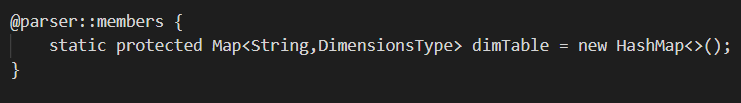
\includegraphics[width=0.75\textwidth]{images/parserdimensions.png}
\caption{Criação do mapa com a informação relativa às dimensões e unidades criadas}
\end{figure}
\par Quanto à gramática em si, trata-se de uma simples lista de instruções que suporta apenas duas, \emph{"dim"} e \emph{"unit"}, usadas para criar dimensões e unidades respetivamente. O funcionamento destas será explicado em detalhe na próxima secção.
\par 
\begin{figure}[h]
\centering
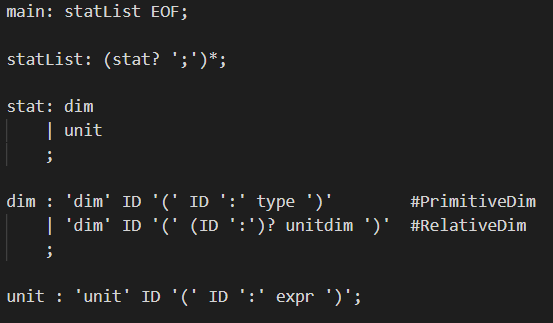
\includegraphics[width=0.5\textwidth]{images/maindimensions.png}
\caption{Parte da gramática correspondente à Linguagem Complementar}
\end{figure}

%%%%%%%%%%%%%%%%%%%%%%%%%%%%%%%%%%%%%%%%%%%%%%%%%%%%%%%%%%%%%%%%%%%%%%%
\clearpage

\subsection{Funcionamento da Linguagem}
\subsubsection{Unidades de Dimensões}
\par Para as unidades das dimensões recorreu-se a dois \emph{HashMaps}, um que possui um \emph{ID} como chave e como valor um \emph{HashMap} representativo da unidade e outro que possui o \emph{ID} dessa mesma unidade como chave e que guarda o seu valor de conversão, em relação à unidade default, como valor.
\par Relativamente ao \emph{HashMap} da unidade, possui como chaves \emph{Strings} correspondentes a cada unidade envolvida, e como valor, o expoente associado a essa unidade. Para comparar se duas unidades pertencem à mesma dimensão verifica-se através da função \emph{equals} entre os \emph{HashMaps} das unidades \emph{default} de cada dimensão.
\par Um outro exemplo de como os \emph{HashMaps} foram úteis, é nas operações de multiplicação, divisão e exponencial.
\par No caso da multiplicação, faz-se um \emph{merge}, em que se as chaves (unidades) forem iguais, soma-se os valores (expoentes) associados, e se forem diferentes, adiciona-os. Depois são removidas todas as chaves que possuírem expoente a zero. 
\begin{figure}[h]
\centering
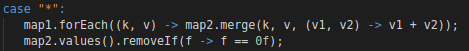
\includegraphics[width=0.75\textwidth]{images/unknown_2.png}
\caption{Parte da multiplicação entre unidades de Dimensões}
\end{figure}
\subsubsection{Criação de nova dimensão}
\par A criação uma nova dimensão pode ser de raiz ou relativa a outras dimensões:

\begin{itemize}
    \item \textbf{De raiz:} \textit{dim [nome]([identificador da unidade base] : [tipo de dados])}
    \item \textbf{Relativa a outras dimensões:} \textit{dim [nome]([operações entre dimensões])}
\end{itemize}

\par O tipo de dados apenas pode ser \textit{Integer} ou \textit{Double} e as operações entre dimensões apenas suportam a multiplicação ou a divisão, sendo que, no caso de alguma dimensão relativa possuir um tipo de dados \textit{Double}, a nova dimensão a ser criada ficará com este tipo. A unidade base da nova dimensão relativa, será a resultante das operações entre as unidades bases das outras dimensões, suportando também as unidades adicionais destas.

\textbf{Como exemplos de utilização:}

\begin{itemize}
    \item \textit{dim Distance(m : Integer);}
    \item \textit{dim Time (s : Double);}
    \item \textit{dim Velocity(Distance/Time);}
\end{itemize}

\subsubsection{Criação de nova unidade}

\par A criação uma nova unidade associada a uma dimensão necessita das operações relativas à unidade base:

\begin{itemize}
    \item \textit{unit [nome da dimensão]([identificador da nova unidade] : [operações relativas a uma unidade da dimensão])}
\end{itemize}

\textbf{Como exemplos de utilização:}

\begin{itemize}
    \item \textit{unit Time(h : 3600*s);}
    \item \textit{unit Velocity(mach: 200*m/s);}
\end{itemize}

%%%%%%%%%%%%%%%%%%%%%%%%%%%%%%%%%%%%%%%%%%%%%%%%%%%%%%%%%%%%%%%%%%%%%%%%%
\subsection{Análise Semântica}

\par A análise semântica é realizada com o \emph{Visitor} denominado \textbf{\emph{DimSemantic.java}}. Este trata de todas as situações que se achou relevantes controlar para que se mantivesse a integridade da linguagem. Segue-se então a lista de regras semânticas que foram incluídas:
\begin{itemize}
    \item Não é permitida a criação de dimensões ou unidades que já existam, no caso das unidades isto é verdade mesmo que em dimensões distintas.
    \item Não é permitido criar uma unidade para uma Dimensão não previamente existente.
    \item Na criação de unidades, a relação que define a mesma não pode incluir unidades pertencentes a outra Dimensão.
    \item Não é permitido criar unidades cuja definição corresponda ao valor 0. 
    \item Na criação de unidades, a relação que define a mesma não pode incluir unidades não definidas previamente.
    \item Na criação de unidades, não é possível elevar uma expressão a uma unidade nem ao valor 0.
\end{itemize}

%%%%%%%%%%%%%%%%%%%%%%%%%%%%%%%%%%%%%%%%%%%%%%%%%%%%%%%%%%%%%%%%%%%%%%%
\newpage
\section{Linguagem Principal}

\par As seguintes secções abordam a linguagem principal do nosso projeto e visam explicar, respectivamente, as bases da implementação em ANTLR4, o funcionamento e sintaxe da linguagem, e ainda a análise semântica desta.

%%%%%%%%%%%%%%%%%%%%%%%%%%%%%%%%%%%%%%%%%%%%%%%%%%%%%%%%%%%%%%%%%%%%%%%
\subsection{Implementação em ANTLR4}

\par Para o funcionamento desta linguagem, foi implementada a gramática \textbf{\textit{chubix.g4}}. Quanto ao parser foram criadas os contadores \emph{"insideLoop"} e \emph{"insideFunc"}, que são efectivamente predicados semânticos relativos a restrições por contexto das instruções iterativas e de funções respectivamente.
\par Adicionalmente foi criada uma \emph{SymbolTable}, classe que visa guardar e interagir com as variáveis criadas, bem como o alcance (\emph{scope}) delas, assimilando uma estrutura em árvore. Para a mesma árvore de \emph{SymbolTables} existem duas referências, sendo que a \emph{"global"} serve como referência para a raiz da árvore e trata do alcance global de um programa e a \emph{"current"} para a \emph{SymbolTable} a ser visitada num dado momento. Portanto, vão existir \emph{SymbolTables} relativas a cada bloco que necessite de variáveis locais (condicionais, iterativos e funções) tendo em conta que a \emph{"current"} tem também acesso às variáveis de todas as tabelas \emph{"parent"} da mesma.
\begin{figure}[h]
\centering
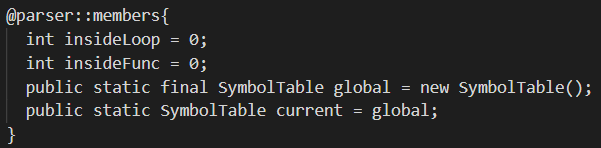
\includegraphics[width=0.75\textwidth]{images/parserchubix.png}
\caption{Criação de variáveis auxiliares à gramática e da tabela de símbolos utilizada no processamento da Linguagem Principal}
\end{figure}
\par Para exemplificar, na análise semântica da linguagem principal, sempre que se entra num bloco de código com um \emph{scope} restrito internamente, é criada uma nova \emph{SymbolTable} filha da \emph{current}, e esta, a \emph{current}, é alterada para se referir à filha criada. Na saída da função é feito um \emph{up}, que coloca a \emph{current} de volta para a \emph{SymbolTable} anterior à entrada na função.
\par No compilador, para respeitar os scopes das variáveis também é feita a mesma estratégia. No entanto, o método que cria uma \emph{SymbolTable} filha é agora substituído por um método que retorna a filha já criada e com os respetivos símbolos guardados. O retorno deste método obedece à ordem de criação das filhas na passagem do \emph{visitor} para a semântica, obtendo assim o resultado pretendido.
\begin{figure}[h]
\centering
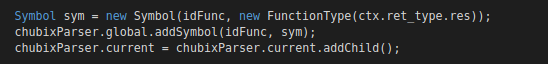
\includegraphics[width=0.75\textwidth]{images/unknown.png}
\caption{Criação de uma nova \textit{SymbolTable} na mudança de \textit{scope}}
\end{figure}
\par A gramática em si baseia-se em três partes do símbolo \emph{main}, primeiramente um cabeçalho opcional de \emph{imports} seguido de um bloco opcional de definição de funções e por fim a lista de instruções que constituem o corpo do programa. Para analisar a gramática completa dirija-se ao ficheiro \textbf{\textit{chubix.g4}}.

\clearpage

\begin{figure}[h]
\centering
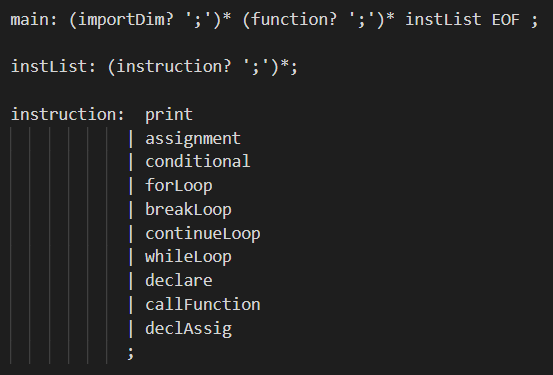
\includegraphics[width=0.5\textwidth]{images/mainchubix.png}
\caption{Parte da gramática correspondente à Linguagem Principal}
\end{figure}

\par É ainda de mencionar, para futura referência, que uma expressão na nossa linguagem pode ser qualquer um dos seguintes:
\begin{itemize}
    \item Uma variável.
	\item Um valor.
	\item Um input.
    \item A chamada a uma função.
	\item Uma variável seguida de incrementação/decrementação.
	\item A conversão de uma expressão.
	\item Uma expressão com sinal (+-).
	\item Uma operação entre expressões, utilizando os operadores aritméticos permitidos (+-*/\string^).
	\item Uma comparação entre expressões, utilizando os operadores relacionais permitidos (== != < > <= >=).
\end{itemize}
\begin{figure}[h]
\centering
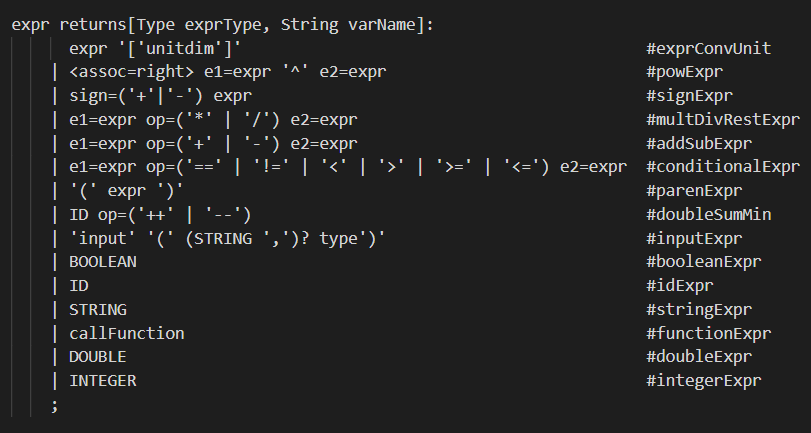
\includegraphics[width=0.565\textwidth]{images/expr.png}
\caption{Implementação em ANTLR4 da expressão}
\end{figure}
%%%%%%%%%%%%%%%%%%%%%%%%%%%%%%%%%%%%%%%%%%%%%%%%%%%%%%%%%%%%%%%%%%%%%%%
\subsection{Funcionamento da Linguagem}

\subsubsection{Importar ficheiros da linguagem complementar}
\par As instruções de importação que forem necessárias incluir no programa têm de ser efectuadas no inicio do mesmo. É possível importar qualquer ficheiro com terminação \emph{.ubi} através do caminho para o mesmo, relativo ao directório do programa.
\textbf{Como exemplos de utilização:}

\begin{itemize}
    \item \textit{import Exemplo.ubi;}
    \item \textit{import ../dic1/dic2/Example.ubi;}
\end{itemize}

\subsubsection{Definição de funções}
\par Todas as funções têm de ser definidas no inicio do programa, mas após as instruções de import, sendo esta a sintaxe a usar:

\begin{lstlisting}[numbers=none]
function <tipo> <nome>(<argumentos>){
    <corpo da funcao>
;}
\end{lstlisting}

\newline
\par \textbf{Tipo:} O tipo de retorno da função, pode ser qualquer um dos existentes (Integer, Double, String, Boolean), qualquer dimensão criada previamente, ou ainda do tipo Void.
\par \textbf{Nome:} O nome atribuído à função, tem de começar por uma letra ou underscore.
\par \textbf{Argumentos:} lista de argumentos da função sob a forma de declarações de variáveis sem valor atribuído.
\par \textbf{Corpo da função:} Lista de instruções que definem a função, tem de incluir uma ou mais instruções de retorno:
\par \textit{return <expressão>;}
\par No caso da função ser do tipo Void a instrução de retorno não inclui expressão.
\newline
\par \textbf{Como exemplo de utilização:}
\begin{lstlisting}[numbers=none]
function Integer Sum(Integer a, Integer b){
    return a + b;
};
\end{lstlisting}


\subsubsection{Declaração de Variáveis}
\par A declaração de variáveis é feita segundo a sintaxe a seguinte:
\begin{lstlisting}[numbers=none]
<tipo> <nome>;
\end{lstlisting}
\newline
\par \textbf{Tipo:} O tipo da variável, pode ser qualquer um dos existentes (Integer, Double, String, Boolean) ou qualquer dimensão criada previamente.
\par \textbf{Nome:} O nome atribuído à variável, tem de começar por uma letra ou underscore.
\newline
\par \textbf{Como exemplos de utilização:}
\begin{itemize}
    \item \textit{Integer a;}
    \item \textit{String s;}
    \item \textit{Time t;}
\end{itemize}

\subsubsection{Atribuição de valor a Variáveis}
\par É possível atribuir valor a uma variável previamente declarada, ou então na declaração de uma, segue-se a sintaxe:
\begin{lstlisting}[numbers=none]
<nome> = <expressao>;
\end{lstlisting}
\par ou então:
\begin{lstlisting}[numbers=none]
<tipo> <nome> = <expressao>;
\end{lstlisting}
\newline
\par É de notar que o tipo da expressão a atribuir tem de se conformar ao tipo da variável, e que no caso da mesma ser dimensional, a expressão deve incluir a unidade a utilizar.
\newline
\par \textbf{Como exemplos de utilização:}
\begin{itemize}
    \item \textit{Velocity v = 10.0 [m/s];}
    \item \textit{Integer a = 10;}
    \item \textit{t = 20 [s];}
    \item \textit{i = a + 5;}
\end{itemize}

\subsubsection{Instrução de Impressão}
\par Para imprimir conteúdo utiliza-se a seguinte instrução:
\begin{lstlisting}[numbers=none]
print(<expressao>);
\end{lstlisting}
\newline
\par \textbf{Como exemplos de utilização:}
\begin{itemize}
    \item \textit{print("Olá!");}
    \item \textit{print(2 [s] + t);}
    \item \textit{print(5.55);}
    \item \textit{print(5 > 2);}
\end{itemize}

\subsubsection{Expressão Input}
\par Embora não seja uma instrução em si, é possível obter dados pelo utilizador através do \emph{input}, relembrando que trata-se apenas de um contexto de expressão. Sendo a sintaxe a seguinte:
\begin{lstlisting}[numbers=none]
input(<texto>, <tipo>);
\end{lstlisting}
\par ou então:
\begin{lstlisting}[numbers=none]
input(<tipo>);
\end{lstlisting}
\newline
\par \textbf{Como exemplos de utilização:}
\begin{itemize}
    \item \textit{Mass m = input("Insira a sua massa em kg",Mass) [kg] ;}
    \item \textit{i = 100 - input(Integer);}
    \item \textit{print(input("Diga o seu nome",String));}
\end{itemize}

\subsubsection{Instrução Condicional}
\par Uma das instruções mais importantes para uma típica linguagem de programação, foi utilizada uma estrutura básica de \emph{if/else}:
\begin{lstlisting}[numbers=none]
if( <expressao> ){
    <lista de instrucoes>
} else if( <expressao> ){
    <lista de instrucoes>
} else{
    <lista de instrucoes>
};
\end{lstlisting}
\newline
\par É de notar que as expressões a passar têm de ser do tipo booleano.
\newline
\par \textbf{Como exemplo de utilização:}
\begin{lstlisting}[numbers=none]
if(num > 0){
    print("Positivo");
} else if (num == 0){
    print("Zero");
} else{
  print("Negativo");
};
\end{lstlisting}

\subsubsection{Instruções Iterativas}
\par Outro tipo de instrução essencial á maior parte das linguagens, no nosso caso implementámos dois blocos simples, a instrução \emph{for} e \emph{while}. Segue-se a sintaxe do ciclo for e while respectivamente:
\begin{lstlisting}[numbers=none]
for( <atribuicao> ; <expressao de termino> ; <incremento> ){
    <lista de instrucoes>
};
\end{lstlisting}
\newline
\par \textbf{Atribuição:} Instrução de atribuição de valor a variável que servirá para controlar o ciclo.
\par \textbf{Expressão de término:} Expressão do tipo booleano que visa definir quando o ciclo deve terminar.
\par \textbf{Incremento:} Instrução de atribuição de valor que dita o tipo de incremento que a variável de controlo vai ter.
\newline
\begin{lstlisting}[numbers=none]
while( <expressao> ){
    <lista de instrucoes>
};
\end{lstlisting}
\newline
\par Quanto ao ciclo while, a expressão passada tem de ser do tipo booleano. Há que mencionar que para ambos os ciclos é possível utilizar as instruções \emph{break;} e \emph{continue;} que terminam o ciclo e ignoram uma iteração respectivamente.
\newline
\par \textbf{Como exemplos de utilização:}
\begin{lstlisting}[numbers=none]
for(Integer i = 0; i<=100; i=i+10){
    print(i*2);
};
\end{lstlisting}
\newline
\begin{lstlisting}[numbers=none]
while(a<b){
    a++;
    b--;
    print("Dentro do ciclo");
};
\end{lstlisting}
%%%%%%%%%%%%%%%%%%%%%%%%%%%%%%%%%%%%%%%%%%%%%%%%%%%%%%%%%%%%%%%%%%%%%%%
\subsection{Análise Semântica}

\par A análise semântica é realizada com o \emph{Visitor} denominado \emph{SemanticChubix.java}. Este trata de todas as situações que se achou relevantes controlar para que se mantivesse a integridade da linguagem. Segue-se então a lista de regras semânticas que foram incluídas:
\begin{itemize}
    \item Não é permitido criar funções com o mesmo nome.
    \item O valor de retorno de uma função tem de se conformar ao tipo da mesma.
    \item Não se pode chamar uma função não definida.
    \item Os argumentos passados na chamada a uma função tem de se conformar aos tipos, ou dimensões se dimensionais, requeridos pela mesma.
    \item O numero de argumentos na chamada de uma função tem de ser igual ao numero de argumentos definidos na mesma.
    \item Não é possível declarar variáveis já existentes no mesmo alcance (\emph{scope}) ou alcances mais abrangentes.
    \item Para atribuir valor a uma variável esta tem de ser previamente declarada.
    \item Ao atribuir valor a uma variável, o valor tem de ser do tipo da variável.
    \item Ao atribuir valor a uma variável dimensional, a sua unidade passada tem de pertencer à dimensão requerida, e o seu valor tem de ser análogo à mesma, havendo excepção se a dimensão for do tipo \emph{double}, e o valor do tipo \emph{integer}.
    \item Numa instrução condicional é necessário passar uma expressão booleana, o mesmo acontece nas condições de instruções iterativas.
    \item Não é permitida a soma de valores pertencentes a dimensões distintas.
    \item É permitida a conversão de expressões numéricas a dimensões, exceptuando se a expressão for do tipo \emph{double} e a dimensão \emph{integer}. 
    \item Não é permitido converter uma expressão dimensional noutra dimensão.
    \item Não é permitido chamar uma função do tipo void no contexto de uma expressão.
    \item Numa expressão não é possível elevar um valor dimensional a um valor não inteiro, ou a zero.
    \item Ao utilizar operadores relacionais, os elementos a comparar devem ser de tipos análogos.
    \item Para utilizar uma variável numa expressão, esta deve estar declarada e com valor atribuído.
\end{itemize}

\clearpage

\section{Geração de Código}

\par Para a compilação e geração de código foi utilizada a ferramenta \textit{String Template} com o objetivo de gerar o código-fonte da linguagem, após a compilação, em \textit{Java}.

\par Terminadas as verificações realizadas na análise semântica, a linguagem procede à compilação através de um visitor, \textit{ChubixComp.java}, onde são introduzidas as instruções passadas pelo utilizador no ficheiro \textit{chubix.stg}, um \textit{STGroupFile} que procede à renderização do \textit{String Template} com o código \textit{Java} final, pronto para ser compilado e executado, de acordo com as regras implementadas pelo grupo.

\par O compilador da linguagem trabalha com o auxílio da tabela de símbolos, preenchida durante a análise semântica, para associar as variáveis criadas durante a compilação com o nome que o utilizador lhes deu, para obter o tipo de dados de variáveis, entre outros. 
Desta forma, é assegurada a compilação de acordo com as verificações feitas previamente. Ao trabalhar com a tabela de símbolos, todas as instruções passadas ao ficheiro \textit{chubix.stg} permitem a compilação sem erros em Java.

\section{Utilização}

\par De modo a permitir a utilização da linguagem desenvolvida, seguem-se instruções para a sua devida utilização:

\begin{itemize}
    \item \textbf{1º - Linguagem Complementar}
    \par Primeiramente é necessário a criação de um ficheiro da linguagem complementar com o formato \textit{.ubi} que permita a definição de Dimensões e das respectivas Unidades de modo a serem utilizadas na Linguagem Principal. 
    \item \textbf{2º - Linguagem Principal}
    \par Após a criação do ficheiro para a Linguagem Complementar, é, também, necessário a criação de um para a Linguagem Principal. O ficheiro deverá estar no formato \textit{.ubix} e deve seguir as regras explicadas previamente, nomeadamente a importação do ficheiro relativo à Linguagem Complementar.
    \item \textbf{3º - Geração do ficheiro Java}
    \par Com os ficheiros de ambas as linguagens prontos, deve-se executar o \textit{Main} da Linguagem Principal com o nome do ficheiro como argumento:
    \begin{lstlisting}[numbers=none]
        java -ea chubixMain [ficheiro da Linguagem Principal]
    \end{lstlisting}
    \par Após esta execução sem erros, é gerado um ficheiro \textit{.java} com o nome do ficheiro da Linguagem Principal utilizado como argumento.
    \item \textbf{4º - Compilação e execução}
    \par Por fim, deve-se compilar o ficheiro \textit{.java} com recurso ao comando \textit{javac} e executá-lo usando o comando \textit{java}. 
\end{itemize}

\par Em caso de necessidade, existem programas exemplo preparados na secção seguinte.

\clearpage

\section{Programas de Exemplo}

\par Nesta secção serão demonstrados alguns exemplos de utilização da linguagem criada. Os programas de exemplo seguintes encontram-se disponíveis dentro da pasta \textit{/tests} na raíz do repositório, sendo que os referentes à Linguagem Complementar encontram-se na pasta \textit{/tests/dimensions} e os referentes à Linguagem Principal em \textit{/tests/chubix}.

\subsection{Programas Corretos}

\subsubsection{Linguagem Complementar}

\par Para o bom funcionamento da Linguagem Principal no seu programa de exemplo correto, todas as dimensões e unidades foram definidas no ficheiro \textit{/tests/dimensions/dimensionsExamples.ubi}:

\begin{lstlisting}[numbers=none]
dim Time(s: Integer);
unit Time(h: 3600*s);

dim Distance(m: Double);
unit Distance(km : 1000*m);

dim Velocity(Distance/Time);
unit Velocity(mach: 200*m/s);

dim Acceleration(Distance/Time^2);

dim Mass(kg: Double);

dim Force(N: Mass*Acceleration);

dim Potential(V: Double);
unit Potential(MV: 10.0^6.0*V);

dim Resistence(O: Double);

dim Current(A: Potential/Resistence);

dim Energy(J: Mass*(Distance^2.5)*Time^-2);

dim Power(W: Energy/Time);
unit Power(KW: W*10.0^3.0);

dim Price(euro : Double);

dim PricePerPowerTime(Price/(Power*Time));

dim Charge(C: Current*Time);

dim IMC(imc : Mass/Distance^2);
\end{lstlisting}

\clearpage

\subsubsection{Linguagem Principal}

\par Após a definição do ficheiro da Linguagem Complementar, foram criados os seguintes exemplos corretos para a Linguagem Principal no ficheiro \textit{/tests/chubix/compilerExamples.ubix}:

\par \textbf{Definição de funções e importação das dimensões e unidades:}

\begin{lstlisting}[numbers=none]
import ../tests/dimensions/dimensionsExamples.ubi;

function Void evalIMC(IMC imc){
    if (imc<16[imc]) {
        print("You are severely underweight.");
    } else if (imc<=19.9[imc]) {
        print("You are underweight.");
    } else if (imc<=24.9[imc]) {
        print("You have a healthy weight.");
    }else if (imc<=29.9[imc]) {
        print("You are overweight.");
    }else if (imc<=39.9[imc]) {
        print("You are obese.");
    }else if (imc>40[imc]) {
        print("You are morbidly obese.");
    };
    return;
};

function Energy CalcCinetica(Velocity v, Mass  m) {
    Energy ec = 0.5*m*v^2;
    return ec;
};

function IMC getIMC(Mass m, Distance height){
    IMC imc = m/height^2;
    return imc;
};
\end{lstlisting}

\par \textbf{Exemplo 1:}

\par Determinar distância percorrida por uma massa de 5kg em 5 segundos.

\begin{lstlisting}[numbers=none]
Time t = 5[s];            
Mass m = 5 [kg];
Velocity v0 = 5[m/s];     
Force f = 5 [kg*m*s^-2];
Acceleration a = f / m;

Distance res = (v0 * t +(a*t^2)/2)[km];

print("Distancia percorrida: ");
print(res);
\end{lstlisting}

\clearpage

\par \textbf{Exemplo 2:}

\par Um circuito elétrico tem uma resistência de o Ohms e uma fonte de tensão de v Volts. Diminuindo a intensidade de corrente para 1/2,1/4...1/32 e mantendo a mesma tensão, pretende-se descobrir o valor em Ohms da nova resistência a aplicar em cada caso.

\begin{lstlisting}[numbers=none]
Potential U =  input("Insira a tensão de corrente em volts", Potential) [V];
Resistence R = input("Insira a intensidade da força, em Newton", Resistence) [O];

Double taxa = 1/2;
Current I = U/R;  # V / O  {'A' : 1, 'V/O' : 1}

while(taxa>=1.0/32.0){
    print("Taxa: ");
    Resistence result = (U/taxa*I^-1) [O];
    print(taxa);
    print("Nova Resistência: ");
    print(result);
    taxa = taxa / 2;
};
\end{lstlisting}

\par \textbf{Exemplo 3:}

\par Determinar a energia consumida mensalmente por um chuveiro elétrico de potência 4000W em uma residência onde vivem quatro pessoas que tomam, diariamente, 2 banhos de 15 min.

\begin{lstlisting}[numbers=none]
Power P = input("Insira a potência: ", Power) [KW];
Time T = input("Insira o tempo da duração de 1 banho: ", Time) [h];

# Da equação da energia consumida temos que E = P x Δt
# Sabendo que são 8 banhos com duração total de 120 min (2h) e considerando os 30 dias do mês, temos:
#   E = 4000 . 2 . 30 = 192.000 = 192 Kwh

Energy E = P * 8 * T * 30;

print("Energia consumida: ");
print(E);
\end{lstlisting}

\par \textbf{Exemplo 3.1:}

\par Na residência pretende-se gastar menos de 30 euros mensalmente com a energia gasta pelo chuveiro. Sabendo que o preço per kWh é de 0.14810 euros, conseguem alcançar este objetivo?

\begin{lstlisting}[numbers=none]
PricePerPowerTime p = input("Preço por kWh: ", PricePerPowerTime) [euro/(KW*h)];

Price p_mensal = p * E;

if (p_mensal < 30[euro]){
    print("Não conseguem gastar menos de 30");
}
else {
    print("Conseguem gastar menos de 30");
};
\end{lstlisting}

\clearpage

\par \textbf{Exemplo 4:}

\par Calcular o a Energia cinética em intervalos de 10s no primeiro minuto do movimento de queda livre. Considere que a velocidade inicial é 0m/s e que a aceleração gravítica é 10m/s\string^2 e que não existem forças de atrito.

\begin{lstlisting}[numbers=none]
Mass m1 = input("Insira a massa do objeto em kg",Mass) [kg] ;
Acceleration g = 10 [m*s^-2];
Velocity v = 0[m/s];
Energy ec;

for (Integer i = 0; i<=60; i=i+10){
    v = v+i[s]*g;
    ec = CalcCinetica(v, m1);
    print(ec); 
};
\end{lstlisting}

\par \textbf{Exemplo 5:}

\par Uma corrente de 5,0 A atravessa um fio durante 4,0 min. Quanto vale (a) a carga que passa por uma secção desse fio e (b) a quantos eletrões corresponde?

\begin{lstlisting}[numbers=none]
#a)

Current cur = 5 [A];
Time time = 4*60 [s];

#Visto que a Intensidade = carga / intervalo de tempo
Charge ch = cur*time ;

print(ch);

#b)

#Número de eletrões = carga / |carga por eletrão|
Double eletroes = ch / (1.602*10^-19)[C];

print(eletroes);
\end{lstlisting}

\par \textbf{Exemplo 6:}

\par Calcular e avaliar o valor de IMC do utilizador.

\begin{lstlisting}[numbers=none]
Mass weight = input("Insert your weight in kg: ", Mass) [kg];
Distance height = input("Insert your height in meters: ", Distance) [m];


IMC imc = getIMC(m,height);
evalIMC(weight/height^2);
\end{lstlisting}

\clearpage

\subsection{Programas com Erros}

\par Foram desenvolvidos alguns programas com erros com o objetivo de verificar se toda a análise semântica da Linguagem funcionava como o esperado. Em cada linha onde é esperado um erro, existe um comentário com o erro.

\subsubsection{Linguagem Complementar}

\begin{lstlisting}[numbers=none]
dim Time(s:Integer);

dim Time2(c:Time);              #[ERROR at line 3] Unit "s" already defined.

unit Time(h: 0 * s);            #[ERROR at line 5] Cannot add a unit with value 0.
unit Time(s: 12*s);             #[ERROR at line 6] Unit "s" already defined.
unit Time(h: 1000);             #[ERROR at line 7] Conversion expression must be a unit.
unit Time(h: s*10);             #[ERROR at line 8 Dimension "Time" and "s^0" are not compatible.

unit Tempo(h : 3600*s);         #[ERROR at line 10] Dimension "Tempo" not defined.

dim Distance(m:Double);

dim Distance(km : Double);      #[ERROR at line 14] Dimension "Distance" already defined.

unit Time(h:3600*m);            #[ERROR at line 16] Dimension "Time" and "3600*m" are not compatible.

unit Distance(cm : 0.01*m);
unit Distance(in: 2.54*cm);     #No error when refering to a unit which is not the default.

dim Velocity(Distance/Time^0);  #[ERROR at line 21] Power of 0 is not possible when defining a dimension.
\end{lstlisting}

\subsubsection{Linguagem Principal}

\begin{lstlisting}[numbers=none]
import ../tests/dimensions/dimensionsExamples.ubi;

function Random CalcCinetica(Velocity v, Mass  m) {#[ERROR at line 3] Dimension "Random" does not exist.
    Energy ec = 0.5*m*v^2;
    return ec;
};

function Energy CalcCinetica(Velocity v, Mass  m) {
    Energy ec = 0.5*m*v^2;
    return ec;
};

function Energy CalcCinetica(Velocity v, Mass  m) {#[ERROR at line 13] Function "CalcCinetica" already exists!
    Energy ec = 0.5*m*v^2;
    return ec;
};


function Void catch(Double x) {
    print(x);
    return;
};

# main

catch(10.0);
catch();                    #[ERROR at line 27] Number of arguments do not match.
CalcCinetica(1 [m], 1 [kg]);#[ERROR at line 28] Incomparable types: m and m / s^1

Distance m = 10;            #[ERROR at line 30] Expression type does not conform to variable "m" type! 
       
Distance m3 = 10[km];       #[ERROR at line 32] There is no dimension with that unit!

Distance m2 = 10[m];
print(m2);

print(m3[m]);                                               
print(m3[s]);               #[ERROR at line 38] Cannot convert to another Dimension!

Time t = 1.2 [s];           #[ERROR at line 40] Cannot convert Double to a Dimension of Integers!

print(catch(10.0) + 1);     #[ERROR at line 42] Expression cannot be void
print("ola"*2);             #[ERROR at line 43] Cannot fetch a type between "ola" and 2

String name = input("Insert your name",String);
Distance r=input("Insert distance in km",Distance)[km];

Distance mm = 1[m];
if(mm>1){                   #[ERROR at line 49] Incomparable types: mm and 1
    print("Maior");
}else{
    print("Menor");
};

Double x = 0;
for (Integer i = 0;i<=2;i=i+1){
    x = 10;
    Integer y = i;
};
print(y);                   #[ERROR at line 60] Variable "y" does not exist!


Integer i = 0;
Integer y = 2;
for (i = 0;i<=2;i=i+1){
    i = 10;
    Integer y = i;          #[ERROR at line 67] Variable "y" already declared!    
};

while(1){                   #[ERROR at line 70] Condition "1" isnt a Boolean expression!
    print("Not boolean");
};

while(true) {
    Double p;
    print(-"hello");        #[ERROR at line 76] Numeric operator applied to a non-numeric operand!
};
Double p;                   #No error

a = 2;

Boolean qwe = p>mm;         #[ERROR at line 82] Variable "p" not defined!
Boolean qwq = 1>mm;         #[ERROR at line 83] Incomparable types: 1 and mm
\end{lstlisting}

\clearpage

\section{Conclusão}

\par Devido à falta de tempo perante as múltiplas entregas que se acumularam no final do semestre, alguns aspetos do trabalho não foram tão bem explorados. A documentação é um exemplo prático deste problema, onde o grupo, perante outras datas de avaliação e cansaço, não conseguiu dedicar o tempo que pretendia inicialmente.

\par Outro fator que se considera ter influenciado negativamente o desenvolvimento do trabalho incide na situação atual que se vive, uma vez que o grupo teve de se adequar a um método de trabalho à distância, algo que anteriormente nunca tinha feito.

\par No geral, a análise semântica foi a parte do trabalho onde se sentiu mais dificuldades, tendo sido necessário a reescrita do código várias vezes após nova análise da documentação do docente.

\par Todos os elementos do grupo concluíram que o desenvolvimento de trabalho favoreceu a compreensão dos tópicos abordados e que será uma mais valia para para a avaliação prática individual.

\par Por fim, acredita-se que todos os objetivos do trabalho foram cumpridos com sucesso.

\section{Contribuições dos autores}
\par Segue-se a contribuição de cada elemento do grupo:
\begin{itemize}
    \item Bruno Bastos -  20\%
	\item Hugo Almeida - 20\%
	\item Mário Silva - 20\%
    \item Leandro Silva - 20\%
	\item Rui Fernandes - 20\%
\end{itemize}

\clearpage

\section{Bibliografia}

\bibliographystyle{plain}

\bibliography{biblist}

\vspace{5mm} %5mm vertical space

[1] Material fornecido pelo docente da disciplina



\end{document}

